\PassOptionsToPackage{unicode=true}{hyperref} % options for packages loaded elsewhere
\PassOptionsToPackage{hyphens}{url}
%
\documentclass[]{article}
\usepackage{lmodern}
\usepackage{amssymb,amsmath}
\usepackage{ifxetex,ifluatex}
\usepackage{fixltx2e} % provides \textsubscript
\ifnum 0\ifxetex 1\fi\ifluatex 1\fi=0 % if pdftex
  \usepackage[T1]{fontenc}
  \usepackage[utf8]{inputenc}
  \usepackage{textcomp} % provides euro and other symbols
\else % if luatex or xelatex
  \usepackage{unicode-math}
  \defaultfontfeatures{Ligatures=TeX,Scale=MatchLowercase}
\fi
% use upquote if available, for straight quotes in verbatim environments
\IfFileExists{upquote.sty}{\usepackage{upquote}}{}
% use microtype if available
\IfFileExists{microtype.sty}{%
\usepackage[]{microtype}
\UseMicrotypeSet[protrusion]{basicmath} % disable protrusion for tt fonts
}{}
\IfFileExists{parskip.sty}{%
\usepackage{parskip}
}{% else
\setlength{\parindent}{0pt}
\setlength{\parskip}{6pt plus 2pt minus 1pt}
}
\usepackage{hyperref}
\hypersetup{
            pdftitle={pop\_gen\_iker},
            pdfborder={0 0 0},
            breaklinks=true}
\urlstyle{same}  % don't use monospace font for urls
\usepackage[margin=1in]{geometry}
\usepackage{color}
\usepackage{fancyvrb}
\newcommand{\VerbBar}{|}
\newcommand{\VERB}{\Verb[commandchars=\\\{\}]}
\DefineVerbatimEnvironment{Highlighting}{Verbatim}{commandchars=\\\{\}}
% Add ',fontsize=\small' for more characters per line
\usepackage{framed}
\definecolor{shadecolor}{RGB}{248,248,248}
\newenvironment{Shaded}{\begin{snugshade}}{\end{snugshade}}
\newcommand{\AlertTok}[1]{\textcolor[rgb]{0.94,0.16,0.16}{#1}}
\newcommand{\AnnotationTok}[1]{\textcolor[rgb]{0.56,0.35,0.01}{\textbf{\textit{#1}}}}
\newcommand{\AttributeTok}[1]{\textcolor[rgb]{0.77,0.63,0.00}{#1}}
\newcommand{\BaseNTok}[1]{\textcolor[rgb]{0.00,0.00,0.81}{#1}}
\newcommand{\BuiltInTok}[1]{#1}
\newcommand{\CharTok}[1]{\textcolor[rgb]{0.31,0.60,0.02}{#1}}
\newcommand{\CommentTok}[1]{\textcolor[rgb]{0.56,0.35,0.01}{\textit{#1}}}
\newcommand{\CommentVarTok}[1]{\textcolor[rgb]{0.56,0.35,0.01}{\textbf{\textit{#1}}}}
\newcommand{\ConstantTok}[1]{\textcolor[rgb]{0.00,0.00,0.00}{#1}}
\newcommand{\ControlFlowTok}[1]{\textcolor[rgb]{0.13,0.29,0.53}{\textbf{#1}}}
\newcommand{\DataTypeTok}[1]{\textcolor[rgb]{0.13,0.29,0.53}{#1}}
\newcommand{\DecValTok}[1]{\textcolor[rgb]{0.00,0.00,0.81}{#1}}
\newcommand{\DocumentationTok}[1]{\textcolor[rgb]{0.56,0.35,0.01}{\textbf{\textit{#1}}}}
\newcommand{\ErrorTok}[1]{\textcolor[rgb]{0.64,0.00,0.00}{\textbf{#1}}}
\newcommand{\ExtensionTok}[1]{#1}
\newcommand{\FloatTok}[1]{\textcolor[rgb]{0.00,0.00,0.81}{#1}}
\newcommand{\FunctionTok}[1]{\textcolor[rgb]{0.00,0.00,0.00}{#1}}
\newcommand{\ImportTok}[1]{#1}
\newcommand{\InformationTok}[1]{\textcolor[rgb]{0.56,0.35,0.01}{\textbf{\textit{#1}}}}
\newcommand{\KeywordTok}[1]{\textcolor[rgb]{0.13,0.29,0.53}{\textbf{#1}}}
\newcommand{\NormalTok}[1]{#1}
\newcommand{\OperatorTok}[1]{\textcolor[rgb]{0.81,0.36,0.00}{\textbf{#1}}}
\newcommand{\OtherTok}[1]{\textcolor[rgb]{0.56,0.35,0.01}{#1}}
\newcommand{\PreprocessorTok}[1]{\textcolor[rgb]{0.56,0.35,0.01}{\textit{#1}}}
\newcommand{\RegionMarkerTok}[1]{#1}
\newcommand{\SpecialCharTok}[1]{\textcolor[rgb]{0.00,0.00,0.00}{#1}}
\newcommand{\SpecialStringTok}[1]{\textcolor[rgb]{0.31,0.60,0.02}{#1}}
\newcommand{\StringTok}[1]{\textcolor[rgb]{0.31,0.60,0.02}{#1}}
\newcommand{\VariableTok}[1]{\textcolor[rgb]{0.00,0.00,0.00}{#1}}
\newcommand{\VerbatimStringTok}[1]{\textcolor[rgb]{0.31,0.60,0.02}{#1}}
\newcommand{\WarningTok}[1]{\textcolor[rgb]{0.56,0.35,0.01}{\textbf{\textit{#1}}}}
\usepackage{graphicx,grffile}
\makeatletter
\def\maxwidth{\ifdim\Gin@nat@width>\linewidth\linewidth\else\Gin@nat@width\fi}
\def\maxheight{\ifdim\Gin@nat@height>\textheight\textheight\else\Gin@nat@height\fi}
\makeatother
% Scale images if necessary, so that they will not overflow the page
% margins by default, and it is still possible to overwrite the defaults
% using explicit options in \includegraphics[width, height, ...]{}
\setkeys{Gin}{width=\maxwidth,height=\maxheight,keepaspectratio}
\setlength{\emergencystretch}{3em}  % prevent overfull lines
\providecommand{\tightlist}{%
  \setlength{\itemsep}{0pt}\setlength{\parskip}{0pt}}
\setcounter{secnumdepth}{0}
% Redefines (sub)paragraphs to behave more like sections
\ifx\paragraph\undefined\else
\let\oldparagraph\paragraph
\renewcommand{\paragraph}[1]{\oldparagraph{#1}\mbox{}}
\fi
\ifx\subparagraph\undefined\else
\let\oldsubparagraph\subparagraph
\renewcommand{\subparagraph}[1]{\oldsubparagraph{#1}\mbox{}}
\fi

% set default figure placement to htbp
\makeatletter
\def\fps@figure{htbp}
\makeatother


\title{pop\_gen\_iker}
\author{}
\date{\vspace{-2.5em}}

\begin{document}
\maketitle

{
\setcounter{tocdepth}{2}
\tableofcontents
}
\hypertarget{introduction-to-the-package}{%
\section{1. Introduction to the
package}\label{introduction-to-the-package}}

\texttt{phasty} is a flexible aand efficient package for using
phase-type theory in R. This vignette describes how to use the
general-purpose phase-type functions for modelling common statistics in
population genomics at the finest level. The formulation of general
phase-type theory can be consulted in Bladt and Nielsen's
`Matrix-Exponential Distributions in Applied Probability', and the
notation for this vignette is also adopted from this book. On the other
hand, the theory behind applying phase-type theory in population
genomics is based on Hobolth et al (2018).

Do not hesitate to run \texttt{?phasty} for a quick summary of the
available general-purpose functions, or to open the help files for the
individual functions.

\begin{Shaded}
\begin{Highlighting}[]
\KeywordTok{library}\NormalTok{(phasty)}
\end{Highlighting}
\end{Shaded}

\hypertarget{continuous-phase-type-distributions-t_mrca-and-t_total}{%
\section{\texorpdfstring{2. Continuous phase-type distributions:
\(T_{MRCA}\) and
\(T_{Total}\)}{2. Continuous phase-type distributions: T\_\{MRCA\} and T\_\{Total\}}}\label{continuous-phase-type-distributions-t_mrca-and-t_total}}

\hypertarget{theoretical-background}{%
\subsection{2.1. Theoretical background}\label{theoretical-background}}

In an evolutionary tree the time until two sequences coalesce \(T_i\)
can be measured in number of generations \(R_i\) divided by the
population size \(N\), this is, \(T_i=R_i/N\). \(T_i\) can easily be
proven to approximate to an exponential distribution with rate
\(\binom{i}{2}\).

In order to understand the evolutionary history of sequences two
additional quantities can be defined --namely the time until the most
recent common ancestor \(T_{MRCA}\) and the total tree length
\(T_{Total}\). \(T_{MRCA}\) will simply be the sum of all times until
two sequences coalesce, in other words \(T_{MRCA}=T_n+T_{n-1}+...+T_2\),
where \(T_i\sim\text{exp}(\binom{i}{2})\). \(T_{Total}\), on the other
hand, takes into account the length of all possible branches, so
\(T_{Total}=nT_n+(n-1)T_{n-1}+...+2T_2\) and, thus,
\(iT_i\sim \text{exp}(\frac{i-1}{2})\).

The mean and variance of these two quantities can be derived relatively
easily. Defining their distribution, however, is more challenging since
both \(T_{MRCA}\) and \(T_{Total}\) are sums of independent
exponentially distributed variables with different rates. Their
distribution can be computed as a series of convolutions, but their
formulation, application and interpretation might be challenging for the
average population geneticist.

Instead, we can think of the sum of exponential distributions as a
continuous-time Markov chain, where coalescent events are represented as
Markov jumps with rate \(T_i\) for \(T_{MRCA}\) and \(iT_i\) for
\(T_{Total}\). The Markov chain will end with an absorbing state, which
in both cases will be the MRCA.

The Markov chain can be represented using phase-type theory, where the
jump rates are defined with a sub-intensity matrix \(T\) and the initial
distribution will be defined as a row vector \(\pi\). If we define
\(\tau\) as the smallest time (or length) to reach the absorbing state,
then \(\tau\sim PH(\pi,T)\). This continuous phase-type distribution has
well-documented and easy-to-implement formulas for the expectation, the
variance, the survival function, the distribution function and the
density function. Moreover, since both \(\pi\) and \(T\) can easily be
speficied, we can represent evolutionary histories that do not follow
the standard coalescent model and still use the same phase-type
formulas.

\texttt{phasty} contains an efficient implementation of continuous
phase-type distributions. This section shows how to create phase-type
representations of \(T_{MRCA}\) and \(T_{Total}\) under the Kingman's
coalescent model, and it provides some guidelines for modeling these
quantities for other non-standard coalescent models.

\hypertarget{time-until-the-most-recent-common-ancestor-t_mrca}{%
\subsection{\texorpdfstring{2.2. Time until the most recent common
ancestor
(\(T_{MRCA}\))}{2.2. Time until the most recent common ancestor (T\_\{MRCA\})}}\label{time-until-the-most-recent-common-ancestor-t_mrca}}

Following Hobolth et al. (2018), we can build a phase-type
representation of \(T_{MRCA}\) by defining the sub-intensity matrix,
which each row and column will represent the states of the coalescent
process.

For example, for Kingman's coalescent the sub-intensity matrix can be
defined as:

\begin{Shaded}
\begin{Highlighting}[]

\NormalTok{subint_mat_t_mrca <-}\StringTok{ }\ControlFlowTok{function}\NormalTok{(n) \{}
  \CommentTok{# Define an matrix filled with zeros}
\NormalTok{  subint_mat <-}\StringTok{ }\KeywordTok{matrix}\NormalTok{(}\KeywordTok{c}\NormalTok{(}\DecValTok{0}\NormalTok{), }\DataTypeTok{nrow =}\NormalTok{ n}\DecValTok{-1}\NormalTok{, }\DataTypeTok{ncol =}\NormalTok{ n}\DecValTok{-1}\NormalTok{)}
  \ControlFlowTok{for}\NormalTok{ (i }\ControlFlowTok{in} \DecValTok{1}\OperatorTok{:}\NormalTok{n}\DecValTok{-1}\NormalTok{) \{}
    \CommentTok{# Save negative exponential rates in the diagonal}
\NormalTok{    subint_mat[i, i] <-}\StringTok{ }\OperatorTok{-}\StringTok{ }\NormalTok{(n }\OperatorTok{-}\StringTok{ }\NormalTok{i}\OperatorTok{+}\DecValTok{1}\NormalTok{)}\OperatorTok{*}\NormalTok{(n }\OperatorTok{-}\StringTok{ }\NormalTok{i)}\OperatorTok{/}\DecValTok{2}
    \ControlFlowTok{if}\NormalTok{ (i }\OperatorTok{<}\StringTok{ }\NormalTok{n}\DecValTok{-1}\NormalTok{) \{}
      \CommentTok{# Define the exponential jumping rates}
\NormalTok{      subint_mat[i, i}\OperatorTok{+}\DecValTok{1}\NormalTok{] <-}\StringTok{ }\OperatorTok{-}\NormalTok{subint_mat[i, i]}
\NormalTok{    \}}
\NormalTok{  \}}
\NormalTok{  subint_mat}
\NormalTok{\}}
\end{Highlighting}
\end{Shaded}

For a sample size of \(n=4\), the sub-intensity matrix can be generated
using the function above, and the initial probabilities can be defined
as a vector of length \(n-1\), starting with one and the rest entries
filled with zeros:

\begin{Shaded}
\begin{Highlighting}[]

\NormalTok{n <-}\StringTok{ }\DecValTok{4}
\NormalTok{subint_mat <-}\StringTok{ }\KeywordTok{subint_mat_t_mrca}\NormalTok{(n)}
\NormalTok{init_probs <-}\StringTok{ }\KeywordTok{matrix}\NormalTok{(}\KeywordTok{c}\NormalTok{(}\DecValTok{1}\NormalTok{, }\KeywordTok{rep}\NormalTok{(}\DecValTok{0}\NormalTok{,n}\DecValTok{-2}\NormalTok{)), }\DecValTok{1}\NormalTok{, n}\DecValTok{-1}\NormalTok{)}
\end{Highlighting}
\end{Shaded}

Now we can use a \texttt{cont\_phase\_type} class of the \texttt{phasty}
package to generate a phase-type representation of \(T_{MRCA}\) by using
\texttt{phase\_type()}:

\begin{Shaded}
\begin{Highlighting}[]

\NormalTok{t_mrca_}\DecValTok{4}\NormalTok{ <-}\StringTok{ }\KeywordTok{phase_type}\NormalTok{(subint_mat, init_probs)}

\NormalTok{t_mrca_}\DecValTok{4}
\CommentTok{#> $subint_mat}
\CommentTok{#>      [,1] [,2] [,3]}
\CommentTok{#> [1,]   -6    6    0}
\CommentTok{#> [2,]    0   -3    3}
\CommentTok{#> [3,]    0    0   -1}
\CommentTok{#> }
\CommentTok{#> $init_probs}
\CommentTok{#>      [,1] [,2] [,3]}
\CommentTok{#> [1,]    1    0    0}
\CommentTok{#> }
\CommentTok{#> $defect}
\CommentTok{#> [1] 0}
\CommentTok{#> }
\CommentTok{#> attr(,"class")}
\CommentTok{#> [1] "cont_phase_type"}
\end{Highlighting}
\end{Shaded}

There are a number of methods associated with the class
\texttt{cont\_phase\_type}. For example, the mean for \(T_{MRCA}\) can
be computed using:

\begin{Shaded}
\begin{Highlighting}[]

\KeywordTok{mean}\NormalTok{(t_mrca_}\DecValTok{4}\NormalTok{)}
\CommentTok{#> [1] 1.5}
\end{Highlighting}
\end{Shaded}

While the variance can be calculated using:

\begin{Shaded}
\begin{Highlighting}[]

\KeywordTok{var}\NormalTok{(t_mrca_}\DecValTok{4}\NormalTok{)}
\CommentTok{#> [1] 1.138889}
\end{Highlighting}
\end{Shaded}

\hypertarget{total-tree-lenght-t_total-and-the-reward-transformation}{%
\subsection{\texorpdfstring{2.3. Total tree lenght (\(T_{Total}\)) and
the
reward-transformation}{2.3. Total tree lenght (T\_\{Total\}) and the reward-transformation}}\label{total-tree-lenght-t_total-and-the-reward-transformation}}

In a similar way to \(T_{MRCA}\), the total tree length or \(T_{Total}\)
can also be represented using phase-type theory (Hobolth et al.~2018).

For Kingman's coalescent the sub-intensity matrix can be defined as:

\begin{Shaded}
\begin{Highlighting}[]

\NormalTok{subint_mat_t_total <-}\StringTok{ }\ControlFlowTok{function}\NormalTok{(n) \{}
\NormalTok{  subint_mat =}\StringTok{ }\KeywordTok{matrix}\NormalTok{(}\KeywordTok{c}\NormalTok{(}\DecValTok{0}\NormalTok{), }\DataTypeTok{nrow =}\NormalTok{ n}\DecValTok{-1}\NormalTok{, }\DataTypeTok{ncol =}\NormalTok{ n}\DecValTok{-1}\NormalTok{)}
  \ControlFlowTok{for}\NormalTok{ (i }\ControlFlowTok{in} \DecValTok{1}\OperatorTok{:}\NormalTok{n}\DecValTok{-1}\NormalTok{) \{}
\NormalTok{    subint_mat[i, i] =}\StringTok{ }\OperatorTok{-}\StringTok{ }\FloatTok{0.5} \OperatorTok{*}\StringTok{ }\NormalTok{(n }\OperatorTok{-}\StringTok{ }\NormalTok{i)}
    \ControlFlowTok{if}\NormalTok{ (i }\OperatorTok{<}\StringTok{ }\NormalTok{n}\DecValTok{-1}\NormalTok{) \{}
\NormalTok{      subint_mat[i, i}\OperatorTok{+}\DecValTok{1}\NormalTok{] =}\StringTok{ }\OperatorTok{-}\NormalTok{subint_mat[i, i]}
\NormalTok{    \}}
\NormalTok{  \}}
\NormalTok{  subint_mat}
\NormalTok{\}}
\end{Highlighting}
\end{Shaded}

For a sample size of \(n=4\), the sub-intensity matrix and the initial
probabilities can be defined as:

\begin{Shaded}
\begin{Highlighting}[]

\NormalTok{n <-}\StringTok{ }\DecValTok{4}
\NormalTok{subint_mat <-}\StringTok{ }\KeywordTok{subint_mat_t_total}\NormalTok{(n)}
\NormalTok{init_probs <-}\StringTok{ }\KeywordTok{matrix}\NormalTok{(}\KeywordTok{c}\NormalTok{(}\DecValTok{1}\NormalTok{, }\KeywordTok{rep}\NormalTok{(}\DecValTok{0}\NormalTok{,n}\DecValTok{-2}\NormalTok{)), }\DecValTok{1}\NormalTok{, n}\DecValTok{-1}\NormalTok{)}
\end{Highlighting}
\end{Shaded}

\(T_{Total}\) can also be represented using the
\texttt{cont\_phase\_type} class:

\begin{Shaded}
\begin{Highlighting}[]

\NormalTok{t_total_}\DecValTok{4}\NormalTok{ <-}\StringTok{ }\KeywordTok{phase_type}\NormalTok{(subint_mat, init_probs)}

\NormalTok{t_total_}\DecValTok{4}
\CommentTok{#> $subint_mat}
\CommentTok{#>      [,1] [,2] [,3]}
\CommentTok{#> [1,] -1.5  1.5  0.0}
\CommentTok{#> [2,]  0.0 -1.0  1.0}
\CommentTok{#> [3,]  0.0  0.0 -0.5}
\CommentTok{#> }
\CommentTok{#> $init_probs}
\CommentTok{#>      [,1] [,2] [,3]}
\CommentTok{#> [1,]    1    0    0}
\CommentTok{#> }
\CommentTok{#> $defect}
\CommentTok{#> [1] 0}
\CommentTok{#> }
\CommentTok{#> attr(,"class")}
\CommentTok{#> [1] "cont_phase_type"}
\end{Highlighting}
\end{Shaded}

Without further ado, we can use the exact same phase-type formulas (and
thus \texttt{phasty} functions) for calculating the mean and variance of
\(T_{Total}\):

\begin{Shaded}
\begin{Highlighting}[]

\KeywordTok{mean}\NormalTok{(t_total_}\DecValTok{4}\NormalTok{)}
\CommentTok{#> [1] 3.666667}
\KeywordTok{var}\NormalTok{(t_total_}\DecValTok{4}\NormalTok{)}
\CommentTok{#> [1] 5.444444}
\end{Highlighting}
\end{Shaded}

\(T_{MRCA}\) and \(T_{total}\) are tightly interconnected. In fact,

\[
T_{total} = T_{MRCA} \circ [n, n-1, ..., 2]
\]

Therefore, \(T_{total}\) can be represented as a reward-transformed
\(T_{MRCA}\), where the reward vector is \([n, n-1, ..., 2]\):

\begin{Shaded}
\begin{Highlighting}[]
\NormalTok{t_total_}\DecValTok{4}\NormalTok{_bis <-}\StringTok{ }\KeywordTok{reward_phase_type}\NormalTok{(t_mrca_}\DecValTok{4}\NormalTok{, }\KeywordTok{c}\NormalTok{(}\DecValTok{4}\NormalTok{, }\DecValTok{3}\NormalTok{, }\DecValTok{2}\NormalTok{))}
\NormalTok{t_total_}\DecValTok{4}\NormalTok{_bis}
\CommentTok{#> $subint_mat}
\CommentTok{#>      [,1] [,2] [,3]}
\CommentTok{#> [1,] -1.5  1.5  0.0}
\CommentTok{#> [2,]  0.0 -1.0  1.0}
\CommentTok{#> [3,]  0.0  0.0 -0.5}
\CommentTok{#> }
\CommentTok{#> $init_probs}
\CommentTok{#>      [,1] [,2] [,3]}
\CommentTok{#> [1,]    1    0    0}
\CommentTok{#> }
\CommentTok{#> $defect}
\CommentTok{#> [1] 0}
\CommentTok{#> }
\CommentTok{#> attr(,"class")}
\CommentTok{#> [1] "cont_phase_type"}
\end{Highlighting}
\end{Shaded}

Which is exactly the same as our previous definition.

\hypertarget{density-distribution-and-quantile-functions}{%
\subsection{2.4. Density, distribution and quantile
functions}\label{density-distribution-and-quantile-functions}}

\texttt{phasty} also includes the density function (\texttt{dphtype()}),
quantile function (\texttt{qphtype()}), distribution function
(\texttt{pphtype()}) and random draw generator (\texttt{rphtype()}) for
continuous phase-type distributions. We can therefore apply these
functions for our phase-type representation of \(T_{MRCA}\) and
\(T_{Total}\).

For example, the density function:

\begin{Shaded}
\begin{Highlighting}[]
\KeywordTok{dphtype}\NormalTok{(}\FloatTok{0.5}\NormalTok{, t_mrca_}\DecValTok{4}\NormalTok{)}
\CommentTok{#> [1] 0.4821092}
\KeywordTok{dphtype}\NormalTok{(}\DecValTok{1}\OperatorTok{:}\DecValTok{3}\NormalTok{, t_total_}\DecValTok{4}\NormalTok{)}
\CommentTok{#> [1] 0.1408529 0.2204939 0.2019975}
\end{Highlighting}
\end{Shaded}

\begin{Shaded}
\begin{Highlighting}[]
\KeywordTok{par}\NormalTok{(}\DataTypeTok{mfrow =} \KeywordTok{c}\NormalTok{(}\DecValTok{1}\NormalTok{, }\DecValTok{2}\NormalTok{))}
\NormalTok{x <-}\StringTok{ }\KeywordTok{seq}\NormalTok{(}\DecValTok{0}\NormalTok{,}\DecValTok{10}\NormalTok{,}\FloatTok{0.1}\NormalTok{)}
\NormalTok{y <-}\StringTok{ }\KeywordTok{dphtype}\NormalTok{(x, t_mrca_}\DecValTok{4}\NormalTok{)}
\KeywordTok{plot}\NormalTok{(x, y, }\DataTypeTok{type =} \StringTok{'l'}\NormalTok{)}
\KeywordTok{lines}\NormalTok{(x, y)}
\KeywordTok{title}\NormalTok{(}\StringTok{'Density function of T_MRCA'}\NormalTok{)}
\NormalTok{x <-}\StringTok{ }\KeywordTok{seq}\NormalTok{(}\DecValTok{0}\NormalTok{,}\DecValTok{20}\NormalTok{,}\FloatTok{0.1}\NormalTok{)}
\NormalTok{y <-}\StringTok{ }\KeywordTok{dphtype}\NormalTok{(x, t_total_}\DecValTok{4}\NormalTok{)}
\KeywordTok{plot}\NormalTok{(x, y, }\DataTypeTok{type =} \StringTok{'l'}\NormalTok{)}
\KeywordTok{lines}\NormalTok{(x, y)}
\KeywordTok{title}\NormalTok{(}\StringTok{'Density function of T_total'}\NormalTok{)}
\end{Highlighting}
\end{Shaded}

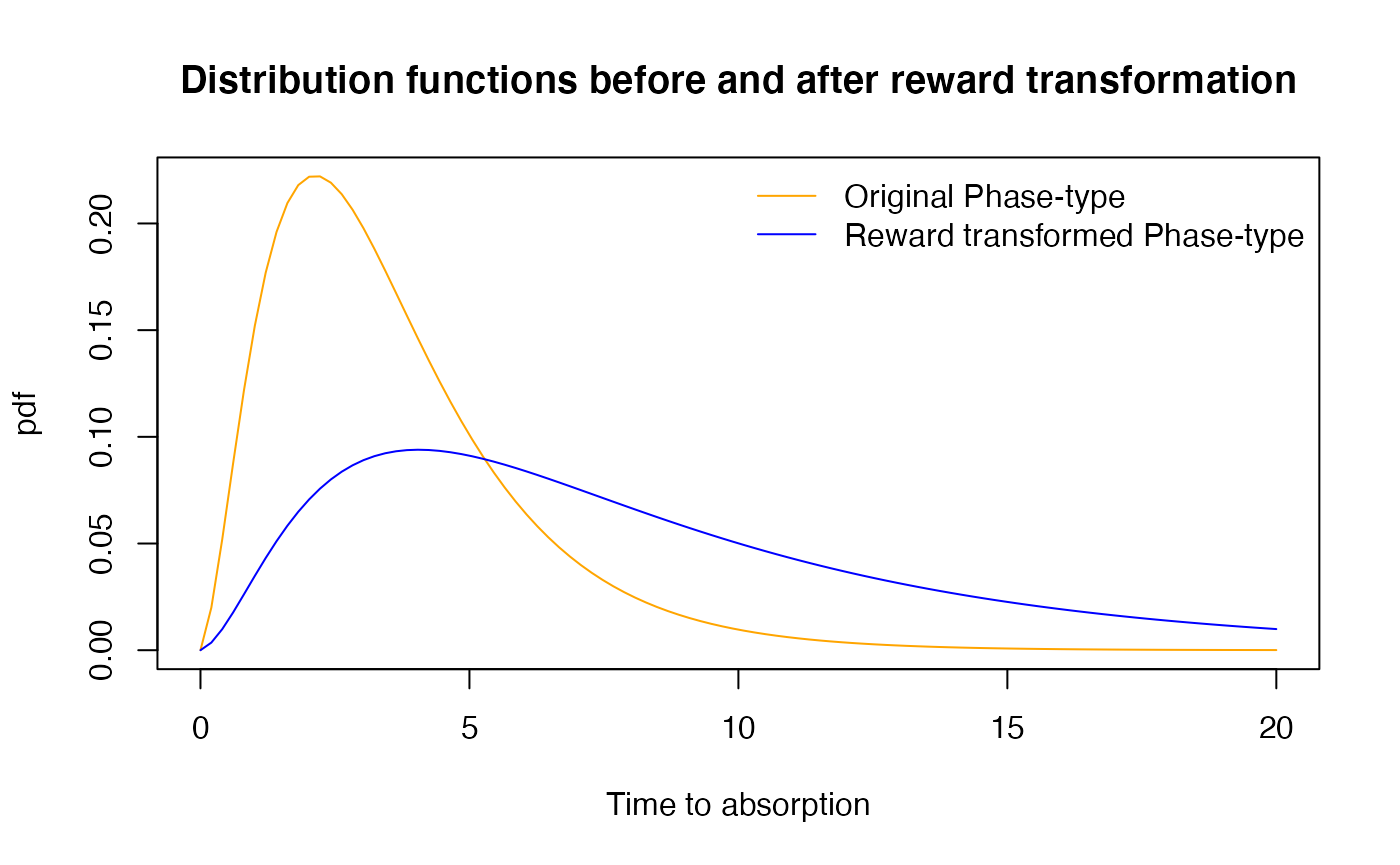
\includegraphics{/Users/au595587/GenomeDK/phasty/vignettes/pop_gen_iker_files/figure-latex/unnamed-chunk-13-1.pdf}

The quantile function:

\begin{Shaded}
\begin{Highlighting}[]
\KeywordTok{qphtype}\NormalTok{(}\FloatTok{0.5}\NormalTok{, t_mrca_}\DecValTok{4}\NormalTok{)}
\CommentTok{#> [1] 1.232831}
\KeywordTok{qphtype}\NormalTok{(}\KeywordTok{c}\NormalTok{(}\FloatTok{0.25}\NormalTok{, }\FloatTok{0.75}\NormalTok{), t_total_}\DecValTok{4}\NormalTok{)}
\CommentTok{#> [1] 1.988284 4.784137}
\end{Highlighting}
\end{Shaded}

\begin{Shaded}
\begin{Highlighting}[]
\KeywordTok{par}\NormalTok{(}\DataTypeTok{mfrow =} \KeywordTok{c}\NormalTok{(}\DecValTok{1}\NormalTok{, }\DecValTok{2}\NormalTok{))}
\NormalTok{x <-}\StringTok{ }\KeywordTok{seq}\NormalTok{(}\DecValTok{0}\NormalTok{,}\FloatTok{0.99}\NormalTok{,}\FloatTok{0.01}\NormalTok{)}
\NormalTok{y <-}\StringTok{ }\KeywordTok{qphtype}\NormalTok{(x, t_mrca_}\DecValTok{4}\NormalTok{)}
\KeywordTok{plot}\NormalTok{(x, y, }\DataTypeTok{type =} \StringTok{'l'}\NormalTok{)}
\KeywordTok{lines}\NormalTok{(x, y)}
\KeywordTok{title}\NormalTok{(}\StringTok{'Quantile function of T_MRCA'}\NormalTok{)}
\NormalTok{x <-}\StringTok{ }\KeywordTok{seq}\NormalTok{(}\DecValTok{0}\NormalTok{,}\FloatTok{0.99}\NormalTok{,}\FloatTok{0.01}\NormalTok{)}
\NormalTok{y <-}\StringTok{ }\KeywordTok{qphtype}\NormalTok{(x, t_total_}\DecValTok{4}\NormalTok{)}
\KeywordTok{plot}\NormalTok{(x, y, }\DataTypeTok{type =} \StringTok{'l'}\NormalTok{)}
\KeywordTok{lines}\NormalTok{(x, y)}
\KeywordTok{title}\NormalTok{(}\StringTok{'Quantile function of T_total'}\NormalTok{)}
\end{Highlighting}
\end{Shaded}

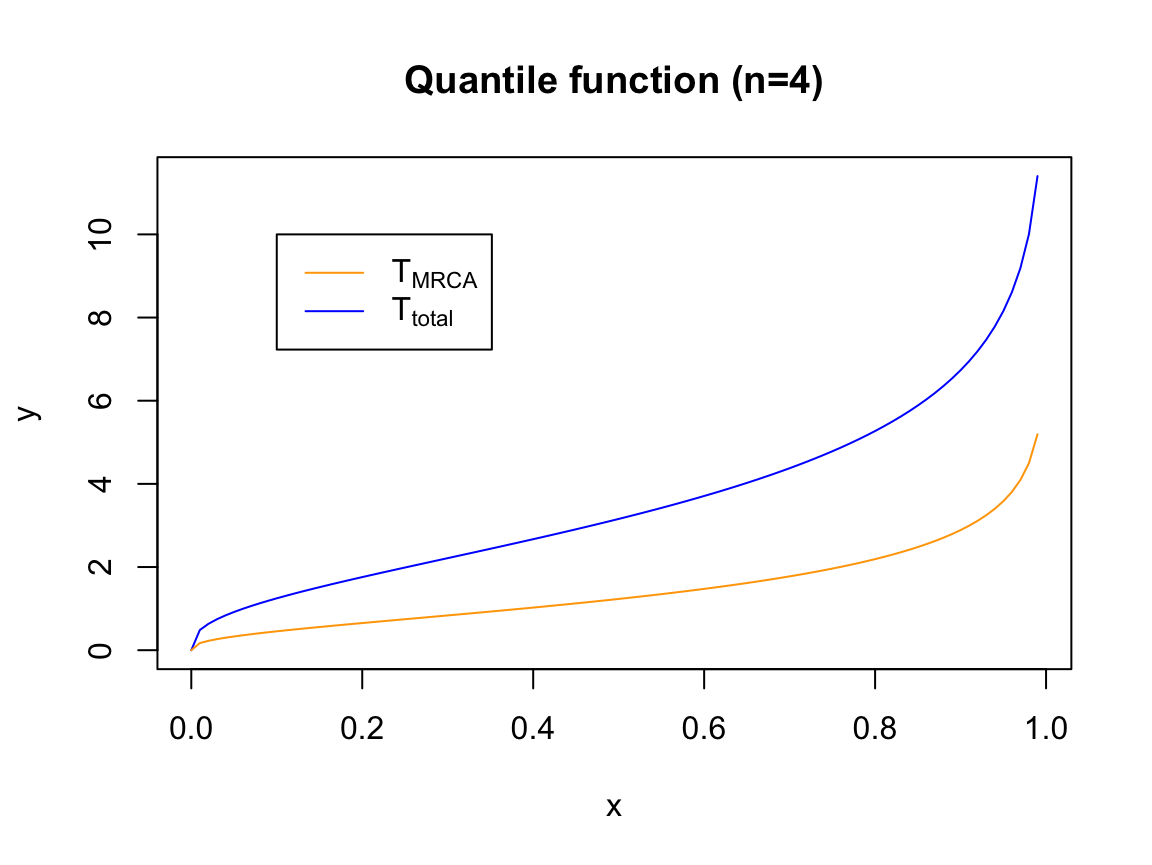
\includegraphics{/Users/au595587/GenomeDK/phasty/vignettes/pop_gen_iker_files/figure-latex/unnamed-chunk-15-1.pdf}

The probability function:

\begin{Shaded}
\begin{Highlighting}[]
\KeywordTok{pphtype}\NormalTok{(}\FloatTok{0.5}\NormalTok{, t_mrca_}\DecValTok{4}\NormalTok{)}
\CommentTok{#> [1] 0.1214176}
\KeywordTok{pphtype}\NormalTok{(}\KeywordTok{c}\NormalTok{(}\FloatTok{0.25}\NormalTok{, }\FloatTok{0.75}\NormalTok{), t_total_}\DecValTok{4}\NormalTok{)}
\CommentTok{#> [1] 0.001622363 0.030579354}
\end{Highlighting}
\end{Shaded}

\begin{Shaded}
\begin{Highlighting}[]
\KeywordTok{par}\NormalTok{(}\DataTypeTok{mfrow =} \KeywordTok{c}\NormalTok{(}\DecValTok{1}\NormalTok{, }\DecValTok{2}\NormalTok{))}
\NormalTok{x <-}\StringTok{ }\KeywordTok{seq}\NormalTok{(}\DecValTok{0}\NormalTok{,}\DecValTok{6}\NormalTok{,}\FloatTok{0.1}\NormalTok{)}
\NormalTok{y <-}\StringTok{ }\KeywordTok{pphtype}\NormalTok{(x, t_mrca_}\DecValTok{4}\NormalTok{)}
\KeywordTok{plot}\NormalTok{(x, y, }\DataTypeTok{type =} \StringTok{'l'}\NormalTok{)}
\KeywordTok{lines}\NormalTok{(x, y)}
\KeywordTok{title}\NormalTok{(}\StringTok{'Probability function of T_MRCA'}\NormalTok{)}
\NormalTok{x <-}\StringTok{ }\KeywordTok{seq}\NormalTok{(}\DecValTok{0}\NormalTok{,}\DecValTok{12}\NormalTok{,}\FloatTok{0.1}\NormalTok{)}
\NormalTok{y <-}\StringTok{ }\KeywordTok{pphtype}\NormalTok{(x, t_total_}\DecValTok{4}\NormalTok{)}
\KeywordTok{plot}\NormalTok{(x, y, }\DataTypeTok{type =} \StringTok{'l'}\NormalTok{)}
\KeywordTok{lines}\NormalTok{(x, y)}
\KeywordTok{title}\NormalTok{(}\StringTok{'Probability function of T_total'}\NormalTok{)}
\end{Highlighting}
\end{Shaded}

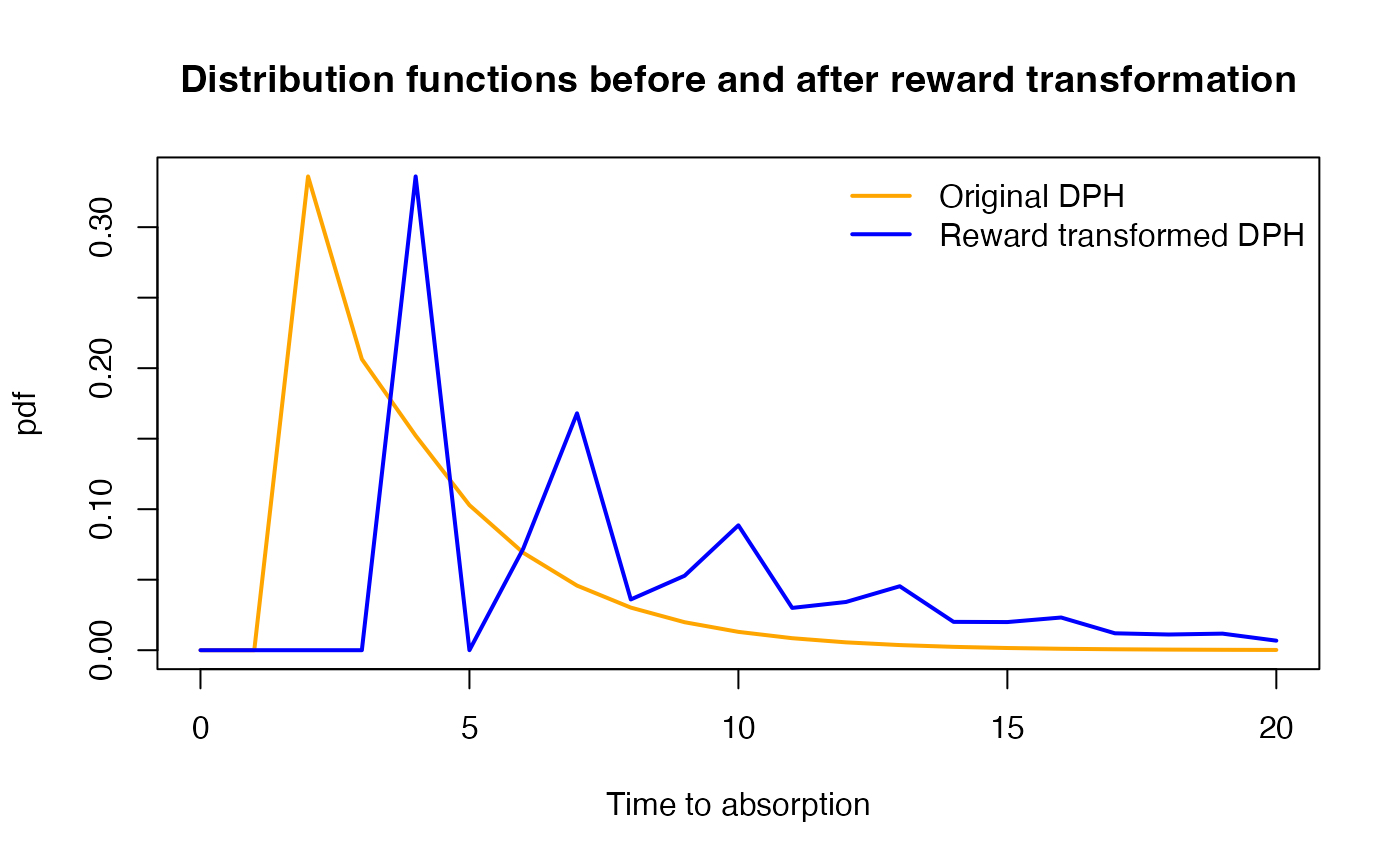
\includegraphics{/Users/au595587/GenomeDK/phasty/vignettes/pop_gen_iker_files/figure-latex/unnamed-chunk-17-1.pdf}

And the random drawer:

\begin{Shaded}
\begin{Highlighting}[]
\KeywordTok{rphtype}\NormalTok{(}\DecValTok{3}\NormalTok{, t_mrca_}\DecValTok{4}\NormalTok{)}
\CommentTok{#> [1] 0.3018729 1.0767638 0.5562144}
\KeywordTok{rphtype}\NormalTok{(}\DecValTok{10}\NormalTok{, t_total_}\DecValTok{4}\NormalTok{)}
\CommentTok{#>  [1] 5.191554 1.905458 1.878108 1.802399 6.561139 3.016019 6.496806 1.643268}
\CommentTok{#>  [9] 3.509529 3.492323}
\end{Highlighting}
\end{Shaded}

\begin{Shaded}
\begin{Highlighting}[]
\KeywordTok{par}\NormalTok{(}\DataTypeTok{mfrow =} \KeywordTok{c}\NormalTok{(}\DecValTok{2}\NormalTok{, }\DecValTok{1}\NormalTok{))}
\NormalTok{x <-}\StringTok{ }\KeywordTok{rphtype}\NormalTok{(}\DecValTok{10000}\NormalTok{, t_mrca_}\DecValTok{4}\NormalTok{)}
\KeywordTok{hist}\NormalTok{(x, }\DataTypeTok{main =} \StringTok{'10,000 random draws of T_MRCA'}\NormalTok{, }\DataTypeTok{breaks=}\DecValTok{50}\NormalTok{)}
\NormalTok{x <-}\StringTok{ }\KeywordTok{rphtype}\NormalTok{(}\DecValTok{10000}\NormalTok{, t_total_}\DecValTok{4}\NormalTok{)}
\KeywordTok{hist}\NormalTok{(x, }\DataTypeTok{main =} \StringTok{'10,000 random draws of T_total'}\NormalTok{, }\DataTypeTok{breaks=}\DecValTok{50}\NormalTok{)}
\end{Highlighting}
\end{Shaded}

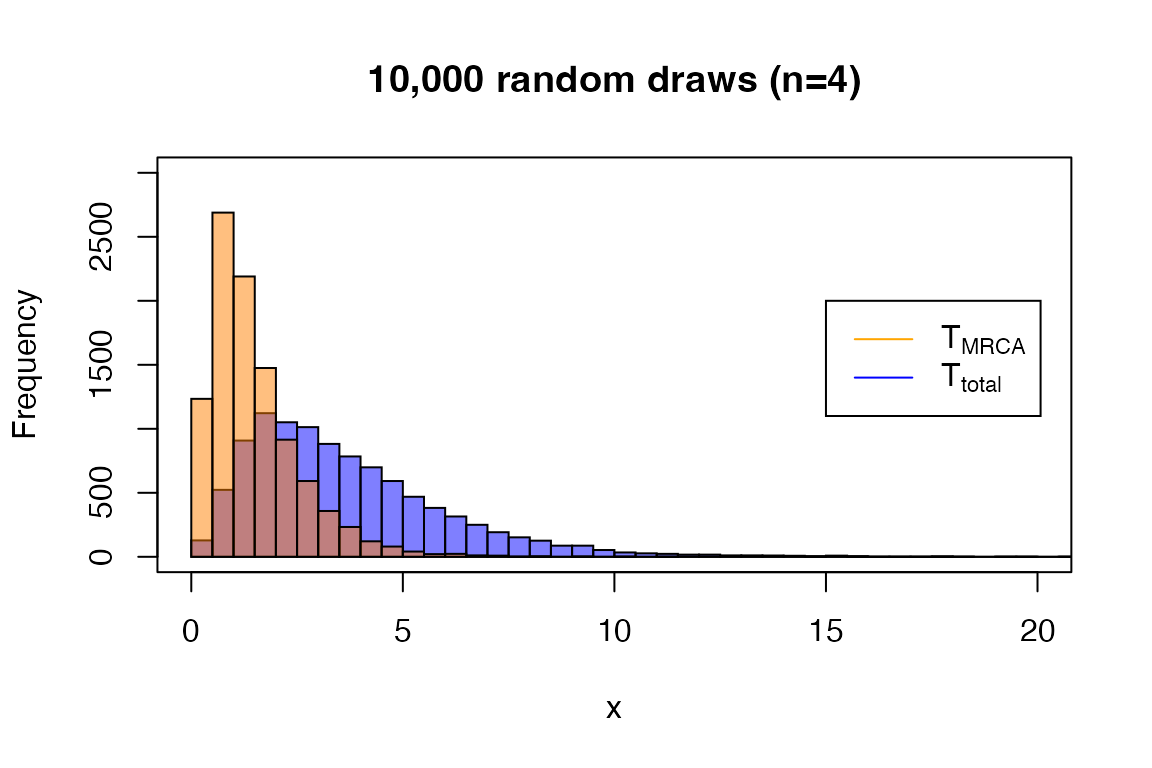
\includegraphics{/Users/au595587/GenomeDK/phasty/vignettes/pop_gen_iker_files/figure-latex/unnamed-chunk-19-1.pdf}

\hypertarget{discrete-phase-type-distributions-s_total-xi_i-and-xi_k}{%
\section{\texorpdfstring{3. Discrete Phase-Type Distributions:
\(S_{total}\), \(\xi_i\) and
\(\xi_{k+}\)}{3. Discrete Phase-Type Distributions: S\_\{total\}, \textbackslash{}xi\_i and \textbackslash{}xi\_\{k+\}}}\label{discrete-phase-type-distributions-s_total-xi_i-and-xi_k}}

\hypertarget{theoretical-background-1}{%
\subsection{3.1. Theoretical
background}\label{theoretical-background-1}}

Some quantities in population genomics are discrete, such as the total
number of segregating sites \(S_{total}\) or other statistics related to
the site-frequency spectrum (singletons, doubletons, tail statistic,
etc.). Representing the site-frequency spectrum, or SFS, can be
challenging if the sample size is large, if the data does not follow
Kingman's coalescence or if we are trying to estimate the mutation
parameter \(\theta\) using non-standard estimators.

Luckily, all these quantities can be represented using discrete
phase-type theory. Similar to the continuous phase-type distribution
being a generalization of exponentially distributed variables, the
discrete phase-type distribution can be seen as a generalization of
various geometric distributions. Each state in the discrete phase-type
distribution will represent a stochastic process, such that the time
until absorption of a random variable (\(\tau\)) follows an absorbing
Markov chain. In this case we say that \(\tau+1\sim DPH(\pi, T)\), where
\(T\) is the sub-intensity matrix that gathers the transition rates and
\(\pi\) is the vector of initial probabilities.

The discrete phase-type representation of \(S_{total}\) can be built
from the continuous phase-type representation of the total branch
length. Folllowing theorem 3.5 in Hobolth et. al (2019), the total
branch length can be discretized if the mutation parameter \(\theta\) is
supplied.

On the other hand, singletons, doubletons and related variables
(referred to as i-tons or \(\xi_i\) throughout this vignette), require a
more elaborate formulation. The idea behind consists in first building a
continuous phase-type representation of the coalescent process, where
the sub-intensity matrix will contain the rates of transition between
all the possible branch types of all possible genealogies. Among all
these branches, only a certain number will give rise to i-tons. We can
calculate which branches these are, together with the weights associated
to each of them. Using this information, we can reward-transform the
continuous phase-type representation of the coalescent process, so it
only represents those branches that give rise to a certain i-ton.
Afterwards, we can discretize this representation using theorem 3.5 in
Hobolth et. al (2019) and the mutation parameter \(\theta\).

Bear in mind that it is possible for some i-tons to never be observed.
This means that the initial probability vector might not sum up to 1,
because the variable might directly jump to the absorbing state. The
probability that this happens is the so-called defect.

Because phase-type theory has well-defined functions for discrete
phase-type distributions, the expectation, the variance, the survival
function, the distribution function and the density function of all the
variables defined above can be computed efficiently. \texttt{phasty}
contains an efficient implementation of discrete phase-type
distributions and all these functions associated to them.

\hypertarget{total-number-of-segregating-sites-s_total}{%
\subsection{\texorpdfstring{3.2. Total number of segregating sites
(\(S_{total}\))}{3.2. Total number of segregating sites (S\_\{total\})}}\label{total-number-of-segregating-sites-s_total}}

As explained above, we can use our previous definition of \(T_{total}\)
and use theorem 3.5 in Hobolth et. al (2018) for a given theta to
discretize the phase-type distribution into the sub-intensity matrix for
\(S_{total}\):

\begin{Shaded}
\begin{Highlighting}[]
\NormalTok{theta <-}\StringTok{ }\DecValTok{3}

\NormalTok{subint_mat <-}\StringTok{ }\NormalTok{t_total_}\DecValTok{4}\OperatorTok{$}\NormalTok{subint_mat}
\NormalTok{init_probs <-}\StringTok{ }\NormalTok{t_total_}\DecValTok{4}\OperatorTok{$}\NormalTok{init_probs}

\NormalTok{disc_subint_mat <-}\StringTok{ }\KeywordTok{solve}\NormalTok{(}\KeywordTok{diag}\NormalTok{(}\KeywordTok{nrow}\NormalTok{(subint_mat)) }\OperatorTok{-}\StringTok{ }\DecValTok{2}\OperatorTok{/}\NormalTok{theta }\OperatorTok{*}\StringTok{ }\NormalTok{subint_mat)}
\end{Highlighting}
\end{Shaded}

And we can now use the \texttt{phase\_type()} function of
\texttt{phasty} to build a discrete phase-type class
\texttt{disc\_phase\_type} for \(S_{total}\):

\begin{Shaded}
\begin{Highlighting}[]

\NormalTok{s_tot_}\DecValTok{4}\NormalTok{_}\DecValTok{3}\NormalTok{ <-}\StringTok{ }\KeywordTok{phase_type}\NormalTok{(disc_subint_mat, init_probs)}
\NormalTok{s_tot_}\DecValTok{4}\NormalTok{_}\DecValTok{3}
\CommentTok{#> $subint_mat}
\CommentTok{#>      [,1] [,2] [,3]}
\CommentTok{#> [1,]  0.5  0.3 0.15}
\CommentTok{#> [2,]  0.0  0.6 0.30}
\CommentTok{#> [3,]  0.0  0.0 0.75}
\CommentTok{#> }
\CommentTok{#> $init_probs}
\CommentTok{#>      [,1] [,2] [,3]}
\CommentTok{#> [1,]    1    0    0}
\CommentTok{#> }
\CommentTok{#> $defect}
\CommentTok{#> [1] 0}
\CommentTok{#> }
\CommentTok{#> attr(,"class")}
\CommentTok{#> [1] "disc_phase_type"}
\end{Highlighting}
\end{Shaded}

The variance and the expectation of any discrete phase-type distribution
can be computed with \texttt{var()} and \texttt{mean()} respectively:

\begin{Shaded}
\begin{Highlighting}[]
\KeywordTok{mean}\NormalTok{(s_tot_}\DecValTok{4}\NormalTok{_}\DecValTok{3}\NormalTok{)}
\CommentTok{#> [1] 6.5}
\KeywordTok{var}\NormalTok{(s_tot_}\DecValTok{4}\NormalTok{_}\DecValTok{3}\NormalTok{)}
\CommentTok{#> [1] 17.75}
\end{Highlighting}
\end{Shaded}

\(S_{total}\) can also be defined in a different way. As suggested by
Hobolth et al.~2018, we can get a matrix that summarizes all the
possible states, each state being a specific combination of i-ton
branches.

As a mock example, we will be using a sample size of \(n=4\), although
the matrix corresponding to an arbitrary sample size can be obtained
using the so-called block-counting process (Hobolth et al.~2018). Using
the standard coalescent model, we can define this matrix as:

\begin{Shaded}
\begin{Highlighting}[]
\NormalTok{subint_itons_}\DecValTok{4}\NormalTok{ <-}\StringTok{ }\KeywordTok{matrix}\NormalTok{(}\KeywordTok{c}\NormalTok{(}\OperatorTok{-}\DecValTok{6}\NormalTok{, }\DecValTok{6}\NormalTok{, }\DecValTok{0}\NormalTok{, }\DecValTok{0}\NormalTok{,}
                           \DecValTok{0}\NormalTok{, }\DecValTok{-3}\NormalTok{, }\DecValTok{2}\NormalTok{, }\DecValTok{1}\NormalTok{,}
                           \DecValTok{0}\NormalTok{, }\DecValTok{0}\NormalTok{, }\DecValTok{-1}\NormalTok{, }\DecValTok{0}\NormalTok{,}
                           \DecValTok{0}\NormalTok{, }\DecValTok{0}\NormalTok{, }\DecValTok{0}\NormalTok{, }\DecValTok{-1}\NormalTok{), }\DataTypeTok{nrow =} \DecValTok{4}\NormalTok{, }\DataTypeTok{byrow =}\NormalTok{ T)}
\end{Highlighting}
\end{Shaded}

And we can also define a continuous phase-type representation of this
process:

\begin{Shaded}
\begin{Highlighting}[]
\NormalTok{kingman_}\DecValTok{4}\NormalTok{ <-}\StringTok{ }\KeywordTok{phase_type}\NormalTok{(subint_itons_}\DecValTok{4}\NormalTok{)}
\CommentTok{#> Warning in phase_type(subint_itons_4): The initial probability vector is}
\CommentTok{#> automatically generated.}
\NormalTok{kingman_}\DecValTok{4}
\CommentTok{#> $subint_mat}
\CommentTok{#>      [,1] [,2] [,3] [,4]}
\CommentTok{#> [1,]   -6    6    0    0}
\CommentTok{#> [2,]    0   -3    2    1}
\CommentTok{#> [3,]    0    0   -1    0}
\CommentTok{#> [4,]    0    0    0   -1}
\CommentTok{#> }
\CommentTok{#> $init_probs}
\CommentTok{#>      [,1] [,2] [,3] [,4]}
\CommentTok{#> [1,]    1    0    0    0}
\CommentTok{#> }
\CommentTok{#> $defect}
\CommentTok{#> [1] 0}
\CommentTok{#> }
\CommentTok{#> attr(,"class")}
\CommentTok{#> [1] "cont_phase_type"}
\end{Highlighting}
\end{Shaded}

And then we must define a reward vector corresponding to each of the
i-tons for each of the states to get a phase-type. In this case:

\begin{Shaded}
\begin{Highlighting}[]
\NormalTok{reward <-}\StringTok{ }\KeywordTok{c}\NormalTok{(}\DecValTok{4}\NormalTok{, }\DecValTok{3}\NormalTok{, }\DecValTok{2}\NormalTok{, }\DecValTok{2}\NormalTok{)}
\NormalTok{seg_sites_cont_}\DecValTok{4}\NormalTok{ <-}\StringTok{ }\KeywordTok{reward_phase_type}\NormalTok{(kingman_}\DecValTok{4}\NormalTok{, reward)}
\NormalTok{seg_sites_cont_}\DecValTok{4}
\CommentTok{#> $subint_mat}
\CommentTok{#>      [,1] [,2]       [,3]       [,4]}
\CommentTok{#> [1,] -1.5  1.5  0.0000000  0.0000000}
\CommentTok{#> [2,]  0.0 -1.0  0.6666667  0.3333333}
\CommentTok{#> [3,]  0.0  0.0 -0.5000000  0.0000000}
\CommentTok{#> [4,]  0.0  0.0  0.0000000 -0.5000000}
\CommentTok{#> }
\CommentTok{#> $init_probs}
\CommentTok{#>      [,1] [,2] [,3] [,4]}
\CommentTok{#> [1,]    1    0    0    0}
\CommentTok{#> }
\CommentTok{#> $defect}
\CommentTok{#> [1] 0}
\CommentTok{#> }
\CommentTok{#> attr(,"class")}
\CommentTok{#> [1] "cont_phase_type"}
\end{Highlighting}
\end{Shaded}

Now we need to discretize this continuous phase-type distribution for
getting the discrete phase-type representation of \(S_{total}\). Using
3.5 in Hobolth et. al (2018):

\begin{Shaded}
\begin{Highlighting}[]
\NormalTok{theta <-}\StringTok{ }\DecValTok{3}

\NormalTok{subint_mat <-}\StringTok{ }\NormalTok{seg_sites_cont_}\DecValTok{4}\OperatorTok{$}\NormalTok{subint_mat}
\NormalTok{init_probs <-}\StringTok{ }\NormalTok{seg_sites_cont_}\DecValTok{4}\OperatorTok{$}\NormalTok{init_probs}

\NormalTok{disc_subint_mat <-}\StringTok{ }\KeywordTok{solve}\NormalTok{(}\KeywordTok{diag}\NormalTok{(}\KeywordTok{nrow}\NormalTok{(subint_mat)) }\OperatorTok{-}\StringTok{ }\DecValTok{2}\OperatorTok{/}\NormalTok{theta }\OperatorTok{*}\StringTok{ }\NormalTok{subint_mat)}

\NormalTok{s_tot_}\DecValTok{4}\NormalTok{_}\DecValTok{3}\NormalTok{_bis <-}\StringTok{ }\KeywordTok{phase_type}\NormalTok{(disc_subint_mat, init_probs)}
\NormalTok{s_tot_}\DecValTok{4}\NormalTok{_}\DecValTok{3}\NormalTok{_bis}
\CommentTok{#> $subint_mat}
\CommentTok{#>      [,1] [,2] [,3] [,4]}
\CommentTok{#> [1,]  0.5  0.3 0.10 0.05}
\CommentTok{#> [2,]  0.0  0.6 0.20 0.10}
\CommentTok{#> [3,]  0.0  0.0 0.75 0.00}
\CommentTok{#> [4,]  0.0  0.0 0.00 0.75}
\CommentTok{#> }
\CommentTok{#> $init_probs}
\CommentTok{#>      [,1] [,2] [,3] [,4]}
\CommentTok{#> [1,]    1    0    0    0}
\CommentTok{#> }
\CommentTok{#> $defect}
\CommentTok{#> [1] 0}
\CommentTok{#> }
\CommentTok{#> attr(,"class")}
\CommentTok{#> [1] "disc_phase_type"}
\end{Highlighting}
\end{Shaded}

This representation seems to differ from the one defined on top, but
they are equivalent in nature. For example, if we look at the mean and
the variance of this new definition:

\begin{Shaded}
\begin{Highlighting}[]
\KeywordTok{mean}\NormalTok{(s_tot_}\DecValTok{4}\NormalTok{_}\DecValTok{3}\NormalTok{_bis)}
\CommentTok{#> [1] 6.5}
\KeywordTok{var}\NormalTok{(s_tot_}\DecValTok{4}\NormalTok{_}\DecValTok{3}\NormalTok{_bis)}
\CommentTok{#> [1] 17.75}
\end{Highlighting}
\end{Shaded}

Because we do not care about the nature of each of the mutations (this
is, we do not care whether segregating sites are singletons, doubletons
or etc.), this way of defining \(S_{total}\) is more inefficient than
the one on top. However, this second definition will be helpful for
getting phase-type representations of i-tons (\(\xi_i\)).

\hypertarget{i-tons-xi_i}{%
\subsection{\texorpdfstring{3.3. i-tons
(\(\xi_i\))}{3.3. i-tons (\textbackslash{}xi\_i)}}\label{i-tons-xi_i}}

The i-tons \(\xi_i\) can also be represented using a discrete phase-type
distribution. We will use the same definition of Kingman's coalescent
process, but this time we need to the reward-transform the continuous
phase-type distribution with a vector corresponding only to the branches
that give rise to a certain \(\xi_i\).

For example, the reward matrix for singletons and the subsequent
continuous phase-type representation of the branches that give rise to
singletons when \(n=4\) (see Hobolth et al.~2018 for further details):

\begin{Shaded}
\begin{Highlighting}[]
\NormalTok{reward <-}\StringTok{ }\KeywordTok{c}\NormalTok{(}\DecValTok{4}\NormalTok{, }\DecValTok{2}\NormalTok{, }\DecValTok{1}\NormalTok{, }\DecValTok{0}\NormalTok{)}
\NormalTok{xi1_cont_}\DecValTok{4}\NormalTok{ <-}\StringTok{ }\KeywordTok{reward_phase_type}\NormalTok{(kingman_}\DecValTok{4}\NormalTok{, reward)}
\NormalTok{xi1_cont_}\DecValTok{4}
\CommentTok{#> $subint_mat}
\CommentTok{#>      [,1] [,2] [,3]}
\CommentTok{#> [1,] -1.5  1.5    0}
\CommentTok{#> [2,]  0.0 -1.5    1}
\CommentTok{#> [3,]  0.0  0.0   -1}
\CommentTok{#> }
\CommentTok{#> $init_probs}
\CommentTok{#>      [,1] [,2] [,3]}
\CommentTok{#> [1,]    1    0    0}
\CommentTok{#> }
\CommentTok{#> $defect}
\CommentTok{#> [1] 0}
\CommentTok{#> }
\CommentTok{#> attr(,"class")}
\CommentTok{#> [1] "cont_phase_type"}
\end{Highlighting}
\end{Shaded}

Again, we need to discretize this continuous phase-type distribution for
getting the discrete phase-type representation of \(\xi_1\). Using 3.5
in Hobolth et. al (2018):

\begin{Shaded}
\begin{Highlighting}[]
\NormalTok{theta <-}\StringTok{ }\DecValTok{3}

\NormalTok{subint_mat <-}\StringTok{ }\NormalTok{xi1_cont_}\DecValTok{4}\OperatorTok{$}\NormalTok{subint_mat}
\NormalTok{init_probs <-}\StringTok{ }\NormalTok{xi1_cont_}\DecValTok{4}\OperatorTok{$}\NormalTok{init_probs}

\NormalTok{disc_subint_mat <-}\StringTok{ }\KeywordTok{solve}\NormalTok{(}\KeywordTok{diag}\NormalTok{(}\KeywordTok{nrow}\NormalTok{(subint_mat)) }\OperatorTok{-}\StringTok{ }\DecValTok{2}\OperatorTok{/}\NormalTok{theta }\OperatorTok{*}\StringTok{ }\NormalTok{subint_mat)}

\NormalTok{xi1_}\DecValTok{4}\NormalTok{_}\DecValTok{3}\NormalTok{ <-}\StringTok{ }\KeywordTok{phase_type}\NormalTok{(disc_subint_mat, init_probs)}
\NormalTok{xi1_}\DecValTok{4}\NormalTok{_}\DecValTok{3}
\CommentTok{#> $subint_mat}
\CommentTok{#>      [,1] [,2] [,3]}
\CommentTok{#> [1,]  0.5 0.25  0.1}
\CommentTok{#> [2,]  0.0 0.50  0.2}
\CommentTok{#> [3,]  0.0 0.00  0.6}
\CommentTok{#> }
\CommentTok{#> $init_probs}
\CommentTok{#>      [,1] [,2] [,3]}
\CommentTok{#> [1,]    1    0    0}
\CommentTok{#> }
\CommentTok{#> $defect}
\CommentTok{#> [1] 0}
\CommentTok{#> }
\CommentTok{#> attr(,"class")}
\CommentTok{#> [1] "disc_phase_type"}
\end{Highlighting}
\end{Shaded}

And we can do the same for doubletons and tripletons:

\begin{Shaded}
\begin{Highlighting}[]
\NormalTok{reward <-}\StringTok{ }\KeywordTok{c}\NormalTok{(}\DecValTok{0}\NormalTok{, }\DecValTok{1}\NormalTok{, }\DecValTok{0}\NormalTok{, }\DecValTok{2}\NormalTok{)}
\NormalTok{xi2_cont_}\DecValTok{4}\NormalTok{ <-}\StringTok{ }\KeywordTok{reward_phase_type}\NormalTok{(kingman_}\DecValTok{4}\NormalTok{, reward)}

\NormalTok{theta <-}\StringTok{ }\DecValTok{3}
\NormalTok{subint_mat <-}\StringTok{ }\NormalTok{xi2_cont_}\DecValTok{4}\OperatorTok{$}\NormalTok{subint_mat}
\NormalTok{init_probs <-}\StringTok{ }\NormalTok{xi2_cont_}\DecValTok{4}\OperatorTok{$}\NormalTok{init_probs}

\NormalTok{disc_subint_mat <-}\StringTok{ }\KeywordTok{solve}\NormalTok{(}\KeywordTok{diag}\NormalTok{(}\KeywordTok{nrow}\NormalTok{(subint_mat)) }\OperatorTok{-}\StringTok{ }\DecValTok{2}\OperatorTok{/}\NormalTok{theta }\OperatorTok{*}\StringTok{ }\NormalTok{subint_mat)}
\NormalTok{xi2_}\DecValTok{4}\NormalTok{_}\DecValTok{3}\NormalTok{ <-}\StringTok{ }\KeywordTok{phase_type}\NormalTok{(disc_subint_mat, init_probs)}
\NormalTok{xi2_}\DecValTok{4}\NormalTok{_}\DecValTok{3}
\CommentTok{#> $subint_mat}
\CommentTok{#>           [,1]      [,2]}
\CommentTok{#> [1,] 0.3333333 0.1666667}
\CommentTok{#> [2,] 0.0000000 0.7500000}
\CommentTok{#> }
\CommentTok{#> $init_probs}
\CommentTok{#>      [,1] [,2]}
\CommentTok{#> [1,]    1    0}
\CommentTok{#> }
\CommentTok{#> $defect}
\CommentTok{#> [1] 0}
\CommentTok{#> }
\CommentTok{#> attr(,"class")}
\CommentTok{#> [1] "disc_phase_type"}
\end{Highlighting}
\end{Shaded}

\begin{Shaded}
\begin{Highlighting}[]
\NormalTok{reward <-}\StringTok{ }\KeywordTok{c}\NormalTok{(}\DecValTok{0}\NormalTok{, }\DecValTok{0}\NormalTok{, }\DecValTok{1}\NormalTok{, }\DecValTok{0}\NormalTok{)}
\NormalTok{xi3_cont_}\DecValTok{4}\NormalTok{ <-}\StringTok{ }\KeywordTok{reward_phase_type}\NormalTok{(kingman_}\DecValTok{4}\NormalTok{, reward)}

\NormalTok{theta <-}\StringTok{ }\DecValTok{3}
\NormalTok{subint_mat <-}\StringTok{ }\NormalTok{xi3_cont_}\DecValTok{4}\OperatorTok{$}\NormalTok{subint_mat}
\NormalTok{init_probs <-}\StringTok{ }\NormalTok{xi3_cont_}\DecValTok{4}\OperatorTok{$}\NormalTok{init_probs}

\NormalTok{disc_subint_mat <-}\StringTok{ }\KeywordTok{solve}\NormalTok{(}\KeywordTok{diag}\NormalTok{(}\KeywordTok{nrow}\NormalTok{(subint_mat)) }\OperatorTok{-}\StringTok{ }\DecValTok{2}\OperatorTok{/}\NormalTok{theta }\OperatorTok{*}\StringTok{ }\NormalTok{subint_mat)}
\NormalTok{xi3_}\DecValTok{4}\NormalTok{_}\DecValTok{3}\NormalTok{ <-}\StringTok{ }\KeywordTok{phase_type}\NormalTok{(disc_subint_mat, init_probs)}
\NormalTok{xi3_}\DecValTok{4}\NormalTok{_}\DecValTok{3}
\CommentTok{#> $subint_mat}
\CommentTok{#>      [,1]}
\CommentTok{#> [1,]  0.6}
\CommentTok{#> }
\CommentTok{#> $init_probs}
\CommentTok{#>           [,1]}
\CommentTok{#> [1,] 0.6666667}
\CommentTok{#> }
\CommentTok{#> $defect}
\CommentTok{#> [1] 0.3333333}
\CommentTok{#> }
\CommentTok{#> attr(,"class")}
\CommentTok{#> [1] "disc_phase_type"}
\end{Highlighting}
\end{Shaded}

And, of course, we can compute the mean and variance for all these
quantities:

\begin{Shaded}
\begin{Highlighting}[]

\KeywordTok{mean}\NormalTok{(xi1_}\DecValTok{4}\NormalTok{_}\DecValTok{3}\NormalTok{)}\OperatorTok{-}\DecValTok{1}\NormalTok{; }\KeywordTok{mean}\NormalTok{(xi2_}\DecValTok{4}\NormalTok{_}\DecValTok{3}\NormalTok{)}\OperatorTok{-}\DecValTok{1}\NormalTok{; }\KeywordTok{mean}\NormalTok{(xi3_}\DecValTok{4}\NormalTok{_}\DecValTok{3}\NormalTok{)}\OperatorTok{-}\DecValTok{1}
\CommentTok{#> [1] 3}
\CommentTok{#> [1] 1.5}
\CommentTok{#> [1] 1}
\KeywordTok{var}\NormalTok{(xi1_}\DecValTok{4}\NormalTok{_}\DecValTok{3}\NormalTok{);  }\KeywordTok{var}\NormalTok{(xi2_}\DecValTok{4}\NormalTok{_}\DecValTok{3}\NormalTok{);  }\KeywordTok{var}\NormalTok{(xi3_}\DecValTok{4}\NormalTok{_}\DecValTok{3}\NormalTok{)}
\CommentTok{#> [1] 7}
\CommentTok{#> [1] 6.75}
\CommentTok{#> [1] 3}
\end{Highlighting}
\end{Shaded}

Note that we need to substract 1 from the mean to retrieve the true
value. This is because of the way discrete phase-type distributions are
defined (see Bladt/Nielsen and Hobolth 2018 for details).

\hypertarget{density-distribution-and-quantile-functions-1}{%
\subsection{3.4. Density, distribution and quantile
functions}\label{density-distribution-and-quantile-functions-1}}

\texttt{phasty} also contains the density function (\texttt{dphtype()}),
quantile function (\texttt{qphtype()}), distribution function
(\texttt{pphtype()}) and random draw generator (\texttt{rphtype()}) for
the discrete phase-type distribution. For example, for \(S_{total}\) and
singletons when \(n=4\) and \(\theta=3\).

For example, the density function:

\begin{Shaded}
\begin{Highlighting}[]
\KeywordTok{dphtype}\NormalTok{(}\DecValTok{4}\NormalTok{, s_tot_}\DecValTok{4}\NormalTok{_}\DecValTok{3}\NormalTok{)}
\CommentTok{#> [1] 0.1197062}
\KeywordTok{dphtype}\NormalTok{(}\DecValTok{1}\OperatorTok{:}\DecValTok{3}\NormalTok{, xi1_}\DecValTok{4}\NormalTok{_}\DecValTok{3}\NormalTok{)}
\CommentTok{#> [1] 0.1500 0.1900 0.1765}
\end{Highlighting}
\end{Shaded}

\begin{Shaded}
\begin{Highlighting}[]
\KeywordTok{par}\NormalTok{(}\DataTypeTok{mfrow =} \KeywordTok{c}\NormalTok{(}\DecValTok{1}\NormalTok{, }\DecValTok{2}\NormalTok{))}
\NormalTok{x <-}\StringTok{ }\DecValTok{1}\OperatorTok{:}\DecValTok{20}
\NormalTok{y <-}\StringTok{ }\KeywordTok{dphtype}\NormalTok{(x, s_tot_}\DecValTok{4}\NormalTok{_}\DecValTok{3}\NormalTok{)}
\KeywordTok{plot}\NormalTok{(x}\DecValTok{-1}\NormalTok{, y, }\DataTypeTok{type =} \StringTok{'l'}\NormalTok{)}
\KeywordTok{lines}\NormalTok{(x}\DecValTok{-1}\NormalTok{, y)}
\KeywordTok{title}\NormalTok{(}\StringTok{'Density function of S_total'}\NormalTok{)}
\NormalTok{x <-}\StringTok{ }\DecValTok{1}\OperatorTok{:}\DecValTok{20}
\NormalTok{y <-}\StringTok{ }\KeywordTok{dphtype}\NormalTok{(x, xi1_}\DecValTok{4}\NormalTok{_}\DecValTok{3}\NormalTok{)}
\KeywordTok{plot}\NormalTok{(x}\DecValTok{-1}\NormalTok{, y, }\DataTypeTok{type =} \StringTok{'l'}\NormalTok{)}
\KeywordTok{lines}\NormalTok{(x}\DecValTok{-1}\NormalTok{, y)}
\KeywordTok{title}\NormalTok{(}\StringTok{'Density function of xi_1'}\NormalTok{)}
\end{Highlighting}
\end{Shaded}

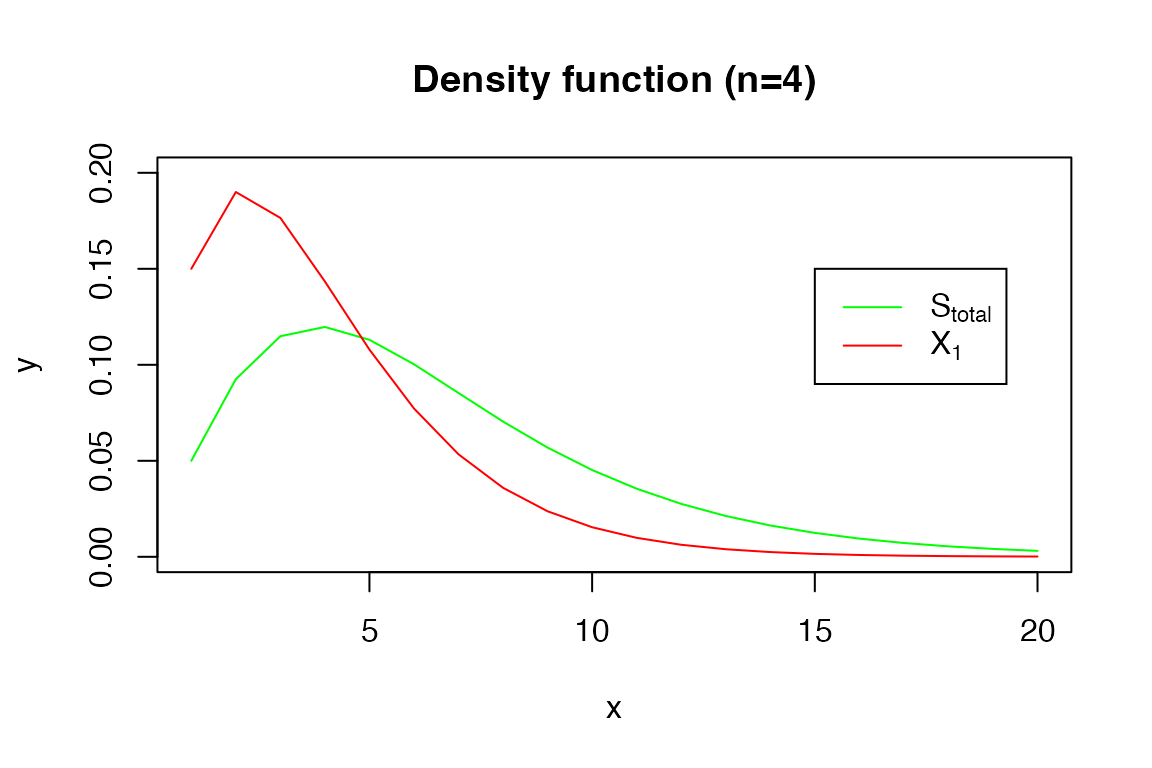
\includegraphics{/Users/au595587/GenomeDK/phasty/vignettes/pop_gen_iker_files/figure-latex/unnamed-chunk-34-1.pdf}

The quantile function:

\begin{Shaded}
\begin{Highlighting}[]
\KeywordTok{qphtype}\NormalTok{(}\FloatTok{0.5}\NormalTok{, s_tot_}\DecValTok{4}\NormalTok{_}\DecValTok{3}\NormalTok{)}
\CommentTok{#> [1] 6}
\KeywordTok{qphtype}\NormalTok{(}\KeywordTok{c}\NormalTok{(}\FloatTok{0.25}\NormalTok{, }\FloatTok{0.75}\NormalTok{), xi1_}\DecValTok{4}\NormalTok{_}\DecValTok{3}\NormalTok{)}
\CommentTok{#> [1] 2 5}
\end{Highlighting}
\end{Shaded}

\begin{Shaded}
\begin{Highlighting}[]
\KeywordTok{par}\NormalTok{(}\DataTypeTok{mfrow =} \KeywordTok{c}\NormalTok{(}\DecValTok{1}\NormalTok{, }\DecValTok{2}\NormalTok{))}
\NormalTok{x <-}\StringTok{ }\KeywordTok{seq}\NormalTok{(}\DecValTok{0}\NormalTok{,}\FloatTok{0.99}\NormalTok{,}\FloatTok{0.01}\NormalTok{)}
\NormalTok{y <-}\StringTok{ }\KeywordTok{qphtype}\NormalTok{(x, s_tot_}\DecValTok{4}\NormalTok{_}\DecValTok{3}\NormalTok{)}
\KeywordTok{plot}\NormalTok{(x, y, }\DataTypeTok{type =} \StringTok{'l'}\NormalTok{)}
\KeywordTok{lines}\NormalTok{(x, y)}
\KeywordTok{title}\NormalTok{(}\StringTok{'Quantile function of S_total'}\NormalTok{)}
\NormalTok{x <-}\StringTok{ }\KeywordTok{seq}\NormalTok{(}\DecValTok{0}\NormalTok{,}\FloatTok{0.99}\NormalTok{,}\FloatTok{0.01}\NormalTok{)}
\NormalTok{y <-}\StringTok{ }\KeywordTok{qphtype}\NormalTok{(x, xi1_}\DecValTok{4}\NormalTok{_}\DecValTok{3}\NormalTok{)}
\KeywordTok{plot}\NormalTok{(x, y, }\DataTypeTok{type =} \StringTok{'l'}\NormalTok{)}
\KeywordTok{lines}\NormalTok{(x, y)}
\KeywordTok{title}\NormalTok{(}\StringTok{'Quantile function of xi_1'}\NormalTok{)}
\end{Highlighting}
\end{Shaded}

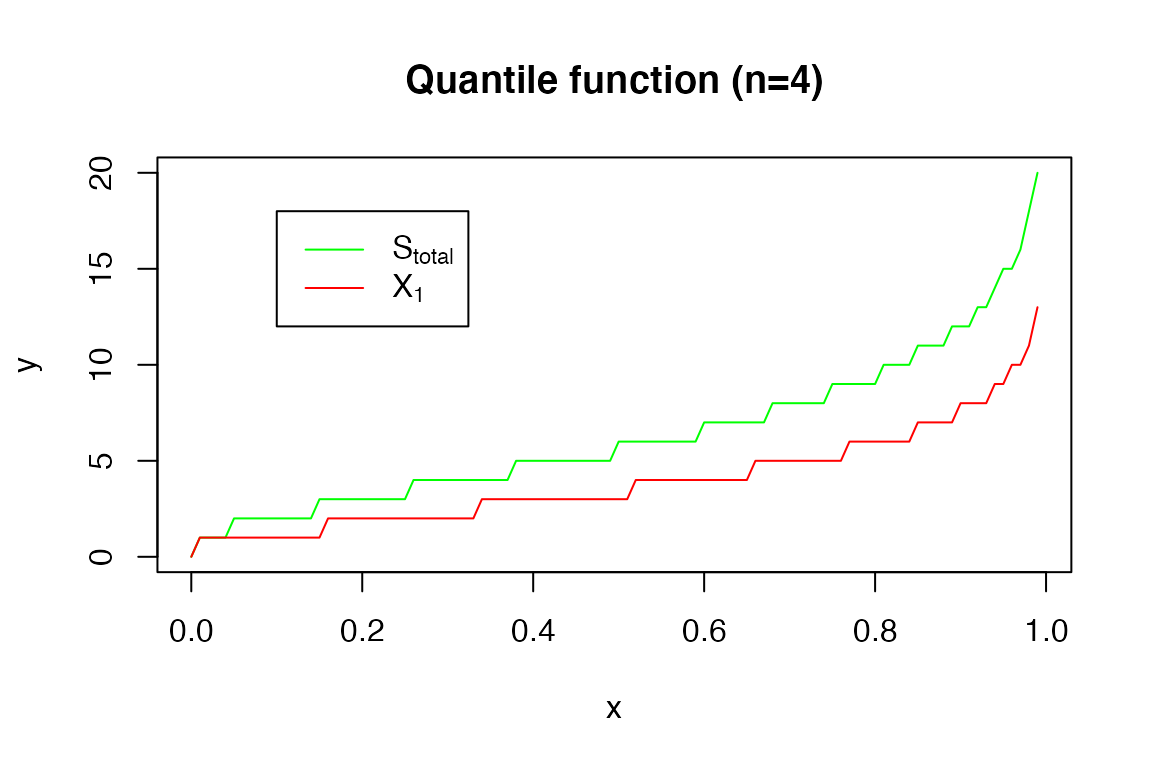
\includegraphics{/Users/au595587/GenomeDK/phasty/vignettes/pop_gen_iker_files/figure-latex/unnamed-chunk-36-1.pdf}

The probability function:

\begin{Shaded}
\begin{Highlighting}[]
\KeywordTok{pphtype}\NormalTok{(}\FloatTok{0.5}\NormalTok{, s_tot_}\DecValTok{4}\NormalTok{_}\DecValTok{3}\NormalTok{)}
\CommentTok{#> [1] 0}
\KeywordTok{pphtype}\NormalTok{(}\KeywordTok{c}\NormalTok{(}\FloatTok{0.25}\NormalTok{, }\FloatTok{0.75}\NormalTok{), xi1_}\DecValTok{4}\NormalTok{_}\DecValTok{3}\NormalTok{)}
\CommentTok{#> [1] 0 0}
\end{Highlighting}
\end{Shaded}

\begin{Shaded}
\begin{Highlighting}[]
\KeywordTok{par}\NormalTok{(}\DataTypeTok{mfrow =} \KeywordTok{c}\NormalTok{(}\DecValTok{1}\NormalTok{, }\DecValTok{2}\NormalTok{))}
\NormalTok{x <-}\StringTok{ }\DecValTok{0}\OperatorTok{:}\DecValTok{20}
\NormalTok{y <-}\StringTok{ }\KeywordTok{pphtype}\NormalTok{(x, s_tot_}\DecValTok{4}\NormalTok{_}\DecValTok{3}\NormalTok{)}
\KeywordTok{plot}\NormalTok{(x, y, }\DataTypeTok{type =} \StringTok{'l'}\NormalTok{)}
\KeywordTok{lines}\NormalTok{(x, y)}
\KeywordTok{title}\NormalTok{(}\StringTok{'Probability function of S_total'}\NormalTok{)}
\NormalTok{x <-}\StringTok{ }\DecValTok{0}\OperatorTok{:}\DecValTok{12}
\NormalTok{y <-}\StringTok{ }\KeywordTok{pphtype}\NormalTok{(x, xi1_}\DecValTok{4}\NormalTok{_}\DecValTok{3}\NormalTok{)}
\KeywordTok{plot}\NormalTok{(x, y, }\DataTypeTok{type =} \StringTok{'l'}\NormalTok{)}
\KeywordTok{lines}\NormalTok{(x, y)}
\KeywordTok{title}\NormalTok{(}\StringTok{'Probability function of xi_1'}\NormalTok{)}
\end{Highlighting}
\end{Shaded}

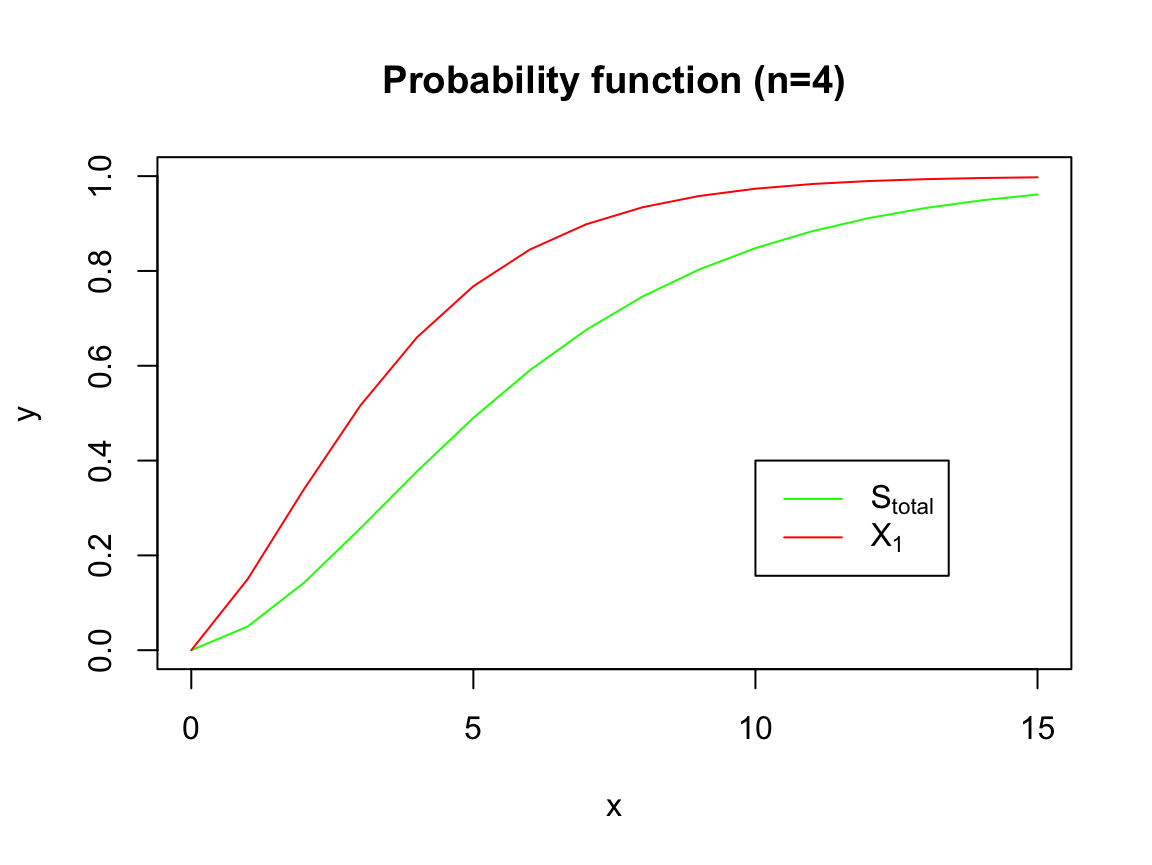
\includegraphics{/Users/au595587/GenomeDK/phasty/vignettes/pop_gen_iker_files/figure-latex/unnamed-chunk-38-1.pdf}

And the random drawer:

\begin{Shaded}
\begin{Highlighting}[]
\KeywordTok{rphtype}\NormalTok{(}\DecValTok{3}\NormalTok{, s_tot_}\DecValTok{4}\NormalTok{_}\DecValTok{3}\NormalTok{)}
\CommentTok{#> [1]  5  8 11}
\KeywordTok{rphtype}\NormalTok{(}\DecValTok{10}\NormalTok{, xi1_}\DecValTok{4}\NormalTok{_}\DecValTok{3}\NormalTok{)}
\CommentTok{#>  [1] 5 1 4 3 4 2 5 2 5 1}
\end{Highlighting}
\end{Shaded}

\begin{Shaded}
\begin{Highlighting}[]
\KeywordTok{par}\NormalTok{(}\DataTypeTok{mfrow =} \KeywordTok{c}\NormalTok{(}\DecValTok{2}\NormalTok{, }\DecValTok{1}\NormalTok{))}
\NormalTok{x <-}\StringTok{ }\KeywordTok{rphtype}\NormalTok{(}\DecValTok{10000}\NormalTok{, s_tot_}\DecValTok{4}\NormalTok{_}\DecValTok{3}\NormalTok{)}\OperatorTok{-}\DecValTok{1}
\KeywordTok{hist}\NormalTok{(x, }\DataTypeTok{main =} \StringTok{'10,000 random draws of S_total'}\NormalTok{, }\DataTypeTok{breaks=}\DecValTok{40}\NormalTok{)}
\NormalTok{x <-}\StringTok{ }\KeywordTok{rphtype}\NormalTok{(}\DecValTok{10000}\NormalTok{, xi1_}\DecValTok{4}\NormalTok{_}\DecValTok{3}\NormalTok{)}\OperatorTok{-}\DecValTok{1}
\KeywordTok{hist}\NormalTok{(x, }\DataTypeTok{main =} \StringTok{'10,000 random draws of xi_1'}\NormalTok{, }\DataTypeTok{breaks=}\DecValTok{20}\NormalTok{)}
\end{Highlighting}
\end{Shaded}

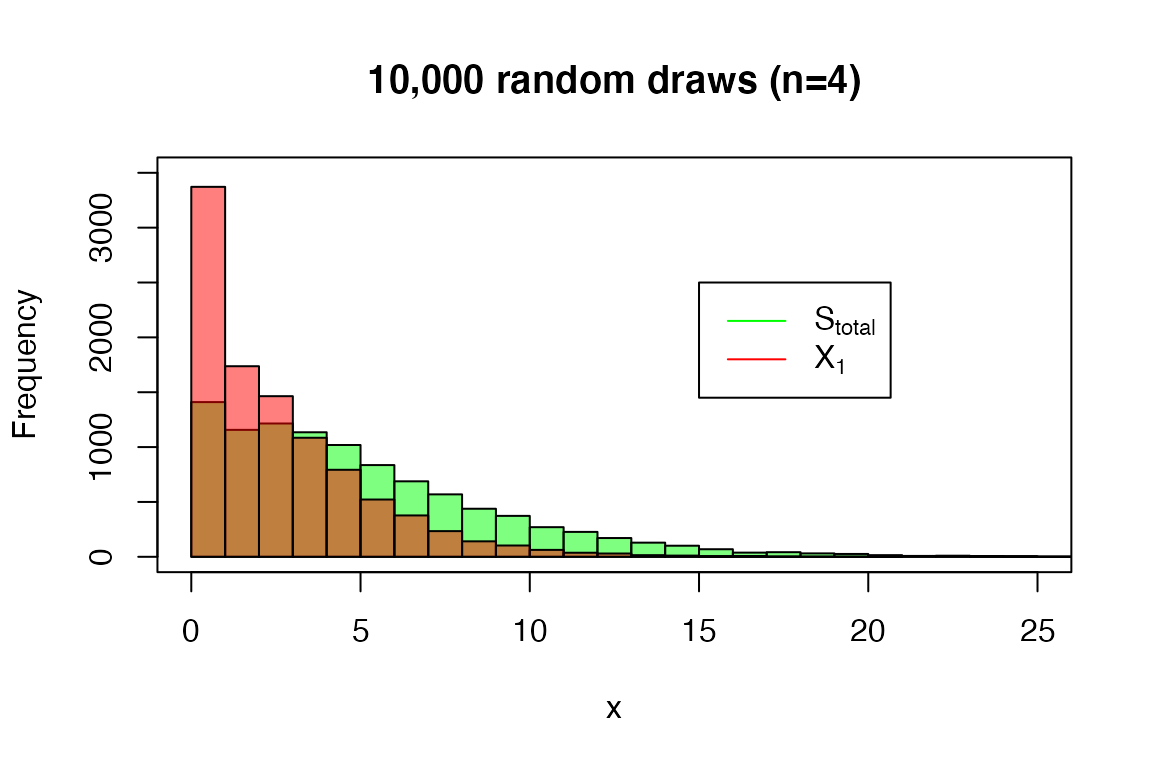
\includegraphics{/Users/au595587/GenomeDK/phasty/vignettes/pop_gen_iker_files/figure-latex/unnamed-chunk-40-1.pdf}

\end{document}
